\label{chap:implementation}

\epigraph{Python is the "most powerful language you can still read".}{\textit{Paul Dubois}}

\section{FANUC robots programming specifics and FANUC software}

\subsection{FANUC Roboguide}

FANUC Roboguide is a proprietary robot simulator and offline programming tool developed by FANUC. Roboguide is in many ways similar to RoboDK.  Like RoboDK, it supports the creation of robot stations, importing of CAD files and CAD-to-path features. The main difference is that Roboguide is limited to FANUC robots and FANUC related technology and procedures. In contrast, RoboDK is not limited to one robot manufactures and is universal and expandable. Roboguide is used for this project to compile the created FANUC programs and upload them to the FANUC robot controller. Roboguide offers several simulation software options tailored for specific robotic arm applications:

\begin{itemize}

\item FANUC Roboguide HandlingPRO - simulating material handling applications including load/unload, packaging, assembly and material removal
\item FANUC Roboguide PaintPRO - simulating painting applications
\item FANUC Roboguide WeldPRO - simulating robotic arc welding process
\item FANUC Roboguide PalletPRO and PalletTool - simulating palletizing applications

\end{itemize}

An example of a Roboguide station is shown in Figure \ref{fig:roboguide}. The version of FANUC Roboguide used for this project is 8.30104.00.35 (Rev. K). 

\begin{figure}[h]
    \centering
    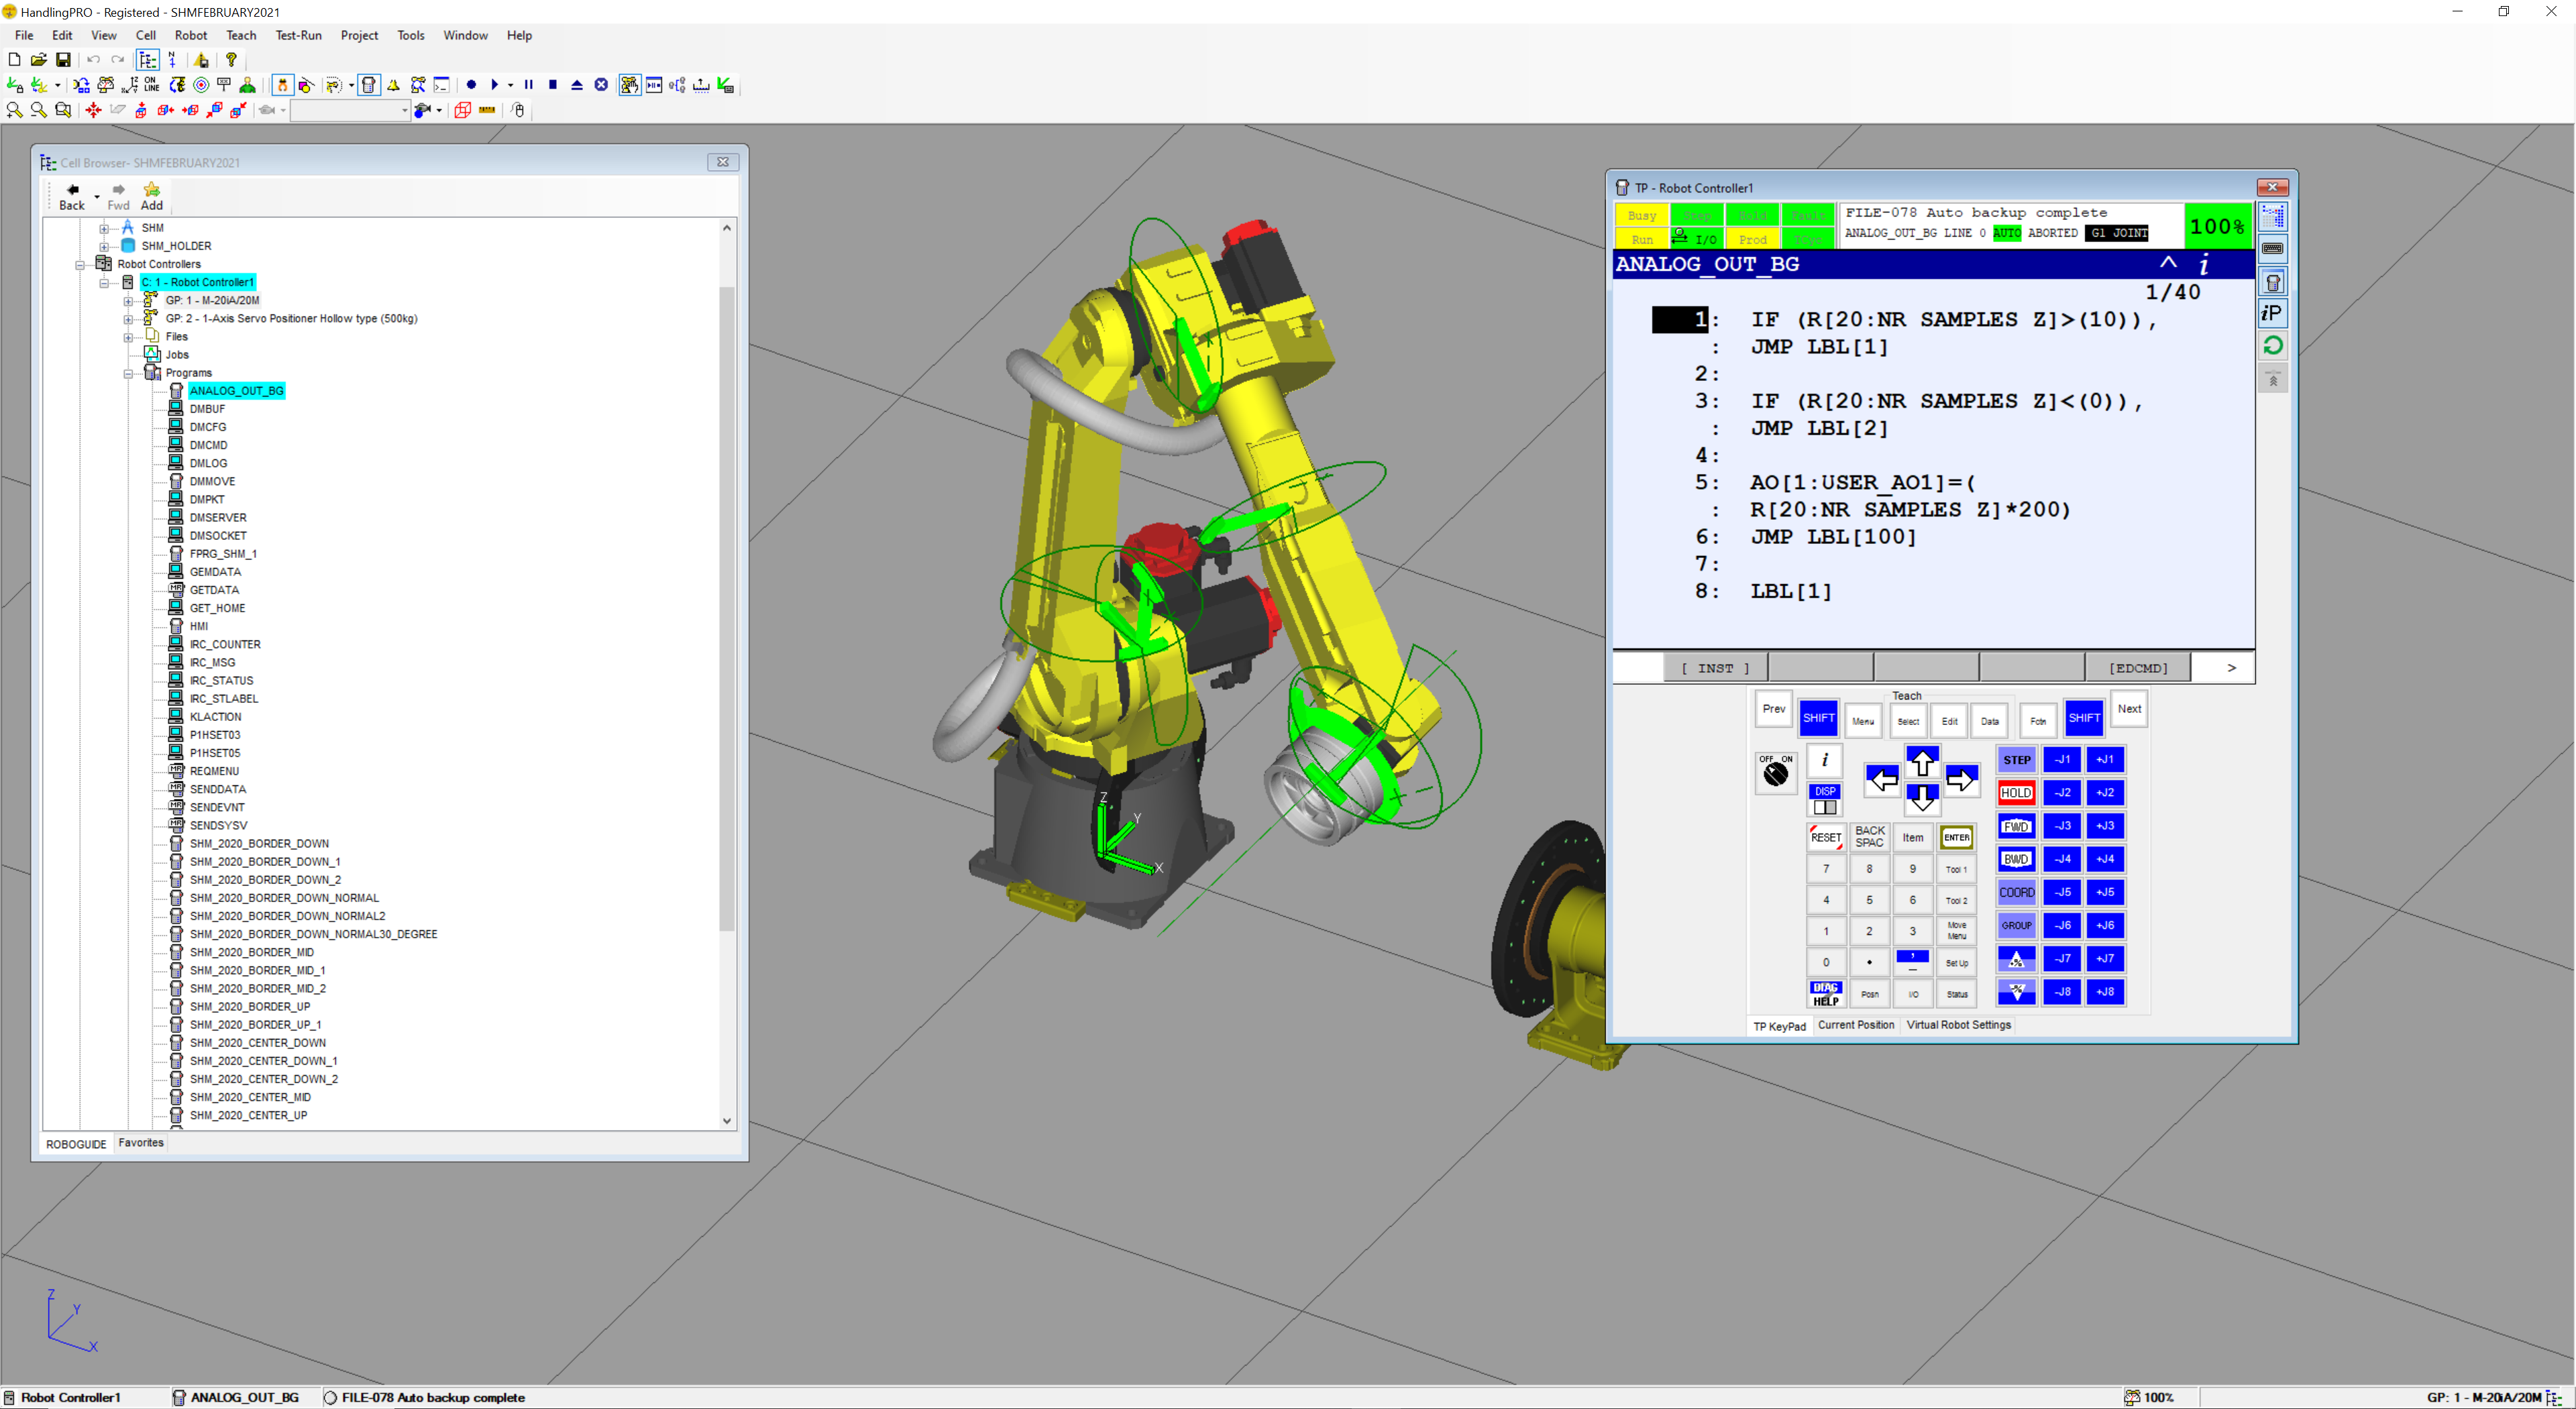
\includegraphics[width=0.9\linewidth]{img/roboguide.PNG}
    \caption{FANUC Roboguide work cell - user interface example.}
    \label{fig:roboguide}
\end{figure}

\subsection{FANUC robot controller programming languages}

The FANUC company implements two programming languages for programming their robot controllers: Teach Pendant (TP) or KAREL. The Teach Pendant language is mainly used for motion control of the robotic arm and edited via the Pendant. Teach pendant programs are either binary files (\mintinline{shell-session}{.tp} file extension) or can be human-readable ASCII files (\mintinline{shell-session}{.ls} file extension). The KAREL language is a high-level language and does not support robot movements. KAREL is mainly used to implement algorithms. KAREL programs can be only edited using a Personal Computer, and they can not be edited using a Pendant.

\subsection{Compiling a FANUC TP program}

Only a Teach Pendant program in binary format can be run on FANUC controllers. Because RoboDK creates TP programs as human-readable ASCII files, the Teach Pendant programs need to be converted to binary format before uploading them to the robot controller. Two options to convert .ls programs to .tp programs exist:

\begin{enumerate}
\item The ASCII Upload option must be loaded on the robot controller. After upload an (\mintinline{shell-session}{.ls} file to the controller it is automatically converted to a (\mintinline{shell-session}{.tp} file.
\item The program is compiled and uploaded either using the WinOLPC  tools via Roboguide or using the WinOLPC tools directly.

\end{enumerate}

\section{Robot machining projects in RoboDK}

The applications of robot machining in the industry are numerous. Some applications include:

\begin{itemize}

    \item milling
    \item drilling
    \item chamfering
    \item deburring

\end{itemize}

RoboDK offers three types of robot manufacturing projects:

\begin{itemize}

    \item Robot machining project
    \item Curve follow project 
    \item Point follow project 

\end{itemize}

This chapter deals with setting up a curve follow project in RoboDK. In laser shock peening, the laser (representing the tool) is static, and the robot holds the object. Therefore, a curve follow project with a constant tool orientation is set up in RoboDK.

\subsection{Setting up a curve follow project in RoboDK}

A curve follow project in RoboDK must at least consist of one robot, one tool and one reference frame. The situation described is a so-called remote TCP situation, i.e. the TCP (Tool Center Point) is fixed in the station, and the robot holds the object. The TCP in our project is represented by the laser source. 
The user has to execute the following steps set up a basic curve follow cell: 

\begin{enumerate}

\item Create and import the path to RoboDK  (using the Load Curves option) path using preferred CAD software. 

\item Mount the robot path as a tool in RoboDK.

\item Create the robotic arm and reference frame (optionally import CAD of object) in RoboDK project. 

\item Create curve follow project: Utilities --> Curve follow project

\item Open the curve follow project settings by double-clicking the project name. A window similar to the one displayed in Figure will open. 

\item In curve follow project settings modify:

    \begin{itemize}

        \item Robot: The station robot holding the object
        \item Reference: The frame representing the remote TCP
        \item Tool: The robot path
        
    \end{itemize}
    
\item Change Select algorithm option to: Robot holds object \& follows path.

\item Update project. RoboDK automatically generates a preprocessed robot program for the actual station.

\item Right-click the preprocessed program, Select Post Processor and Generate program. The .ls program for the actual station will be opened in the default RoboDK text editor.

\item Compile the program and export the program to the FANUC robot controller using Roboguide or WinOLPC tools.
    
\end{enumerate}

\begin{figure}[h]
    \centering
    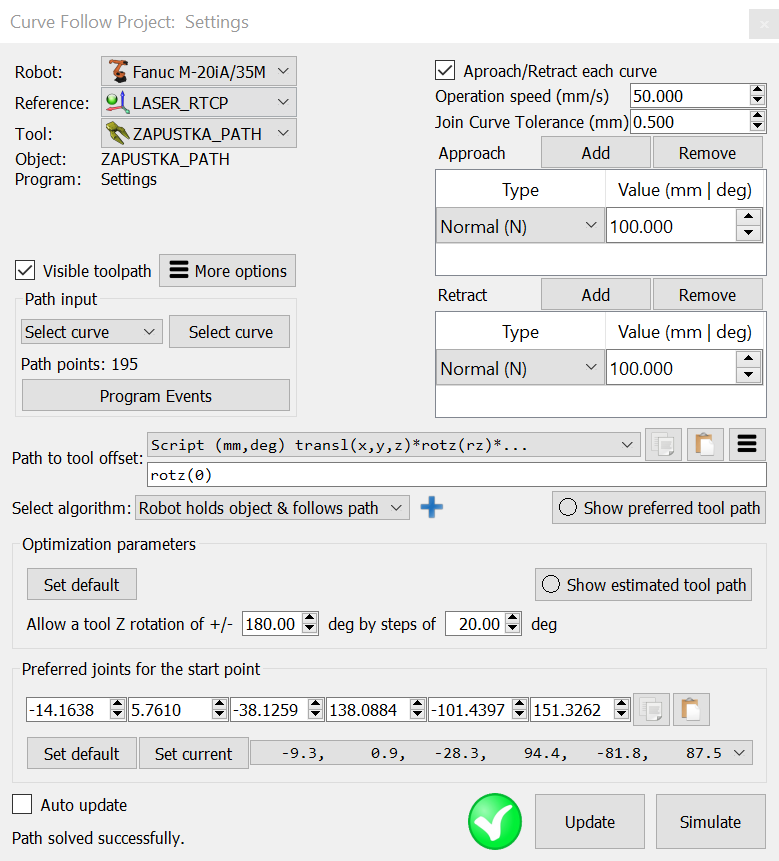
\includegraphics[width=0.9\linewidth]{img/curve_follow_settings.PNG}
    \caption{Curve follow project settings in RoboDK.}
    \label{fig:curvefollow}
\end{figure}

\section{RoboDK API for Python}

\section{Installation, Python setup and path settings of RoboDK API}

\section{Post processors}

\subsection{RoboDK post processors overview}

A post processor specifies how robot programs must be generated for a specific robot controller. Post processors serve as tools to convert the simulation to vendor-specific robot programs. All RoboDK post processors are placed in the \mintinline{shell-session}{C:/RoboDK/Posts/} folder in the Windows operating system. Post processors rely on the \mintinline{shell-session}{robodk} module. The \mintinline{shell-session}{robodk} module is a robotics toolbox for Python, based on \href{http://petercorke.com/Robotics_Toolbox.html}{Peter Corke’s Robotics Toolbox}. 

\subsection{FANUC R-30iA post processor}

The FANUC R-30iA post processor is located in the \mintinline{shell-session}{C:/RoboDK/Posts/vXX folder}. \mintinline{shell-session}{XX} is a two-digit number and denotes the post processor version. The FANUC R-30iA post processor comes in the form of a \mintinline{shell-session}{.pyc} file (compiled bytecode) and needs to be decompiled to a \mintinline{shell-session}{.py} file with the help of a decompiler. The decompyler used in this thesis is   \href{https://github.com/rocky/python-decompile3}{decompyle3}.

When a program is generated, a preprocessed/universal Python program is generated and saved in a local temporary folder. The preprocessed program is linked with the right post processor (selected by the user in RoboDK). The post processor defines a \mintinline{shell-session}{RobotPost} class that generates the desired code. On Windows, the preprocessed Python files are saved in the user's temporary folder (for example: \mintinline{shell-session}{C:/Users/username/AppData/Local/Temp folder}). These programs can also be used for debugging new post processors.


\section{Modifying a post processor}


